\chapter{Drónvezérlést tesztelő környezetek}
\label{chap:vmtest}

\section{Képfelismerésen alapuló drónvezérlő automatizált drónvezérlő scenario}
\label{cha:fizikai}
A diplomatervezés második félévére továbbfejlődött a projekt, aminek integrálása a feladatom, így a \ref{chap:vmtest}. fejezetben taglaltaknál egy komplexebb rendszert is kialakíthatunk, de továbbra is a már tesztelt négy konténeren alapszik a megoldásom. Azonban ebben a fejezetben megnézem, hogyan néz ki a felhő nélküli, egy gépen, konténereken megvalósított megoldás. A fejlesztéshez kaptam egy \emph{drone-control-2} nevű könyvtárat, ami egy docker-compose.yaml fájlt és a hozzá tartozó Docker konténerek alkönyvtárait tartalmazza. A féléves munkám során készített kódbázis feltétele, hogy a gyökörkönyvtár szülője tartalmazza a drone-control-2 nevű projektet vagyis annak a 2020 november harmadikán módosított változtatát. \\

\noindent
A földön használt rendszer a következő komponensekből áll:
\begin{itemize}
	\item Fizikai drón
	\item GCS kommunikációs eszköz
	\item VKE irányítóközpont
\end{itemize}

\noindent
A GCS eszköz valósítja meg a közeghozzáférést a fizikai drónnak, amin keresztül csatlakozik a hálózathoz. Ezt a közeghozzáférési technológiát nem elemezzük, azonban feljegyezzük, hogy ebben a kiépített rendszerben a vezérlőfelületen kiadott parancs a drónhoz $T_{GCS} = ~300 ms$ késleltetés idő alatt kezdi meg a végrehajtását. \\

\noindent
A VKE irányítóközpont felel minden feldolgozandó és irányítandó tényezőről, továbbá a felhasználói interfészről is. A kész VKE rendszer blokkdiagramja a \ref{fig:vke}. ábrán látható. A kék háttér mögött minden komponens Docker konténerben fut és hostname-ek alapján kommunikál. A komponensek a következő feladatokat látják el:
\begin{itemize}
	\item Tunnel: bevezeti kívülről a Mavlink és a HTTP kommunikációt
	\item Roscore: A ROS számításait végzi
	\item Mavros irányítópult: A felhasználói interfész és az irányítás megvalósítása
	\item Videó feldolgozó: A drón kamerájából érkező jelet fogadja
	\item Aruco képfeldolgozó: Az Aruco kódokat detektálja a kamerajelen
	\item AI: A kamerakép mesterséges intelligencia alapú feldolgozása
	\item Map: Az aruco kódok alapján parancsokat ad ki
\end{itemize}

\begin{figure}
	\centering
	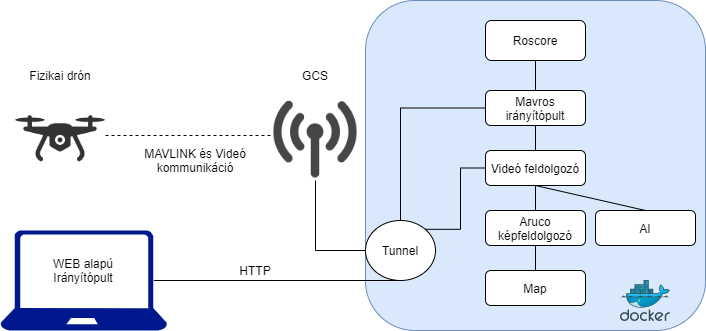
\includegraphics[width=\linewidth]{figures/vke_drone.png}
	\caption{Kész VKE földi rendszer}
	\label{fig:vke}
\end{figure}

\noindent
Ezen bemutatott rendszer az amit felhőbe integrálok, fizikai drón helyett szimulációval és leegyszerűsítve a funkciókat és a hálózati megvalósítást. A négy konténer amivel tovább dolgozom, az a Roscore, Mavros irányítópult, Aruco képfeldolgozó és ami a \ref{fig:vke}. számú ábrán nincs rajta, a PX4 alapú Gazebo szimuláció konténere. Az ábrán látható konténerek mindegyike Docker technológiával megvalósított és a \emph{drone-control-2} gyűjtőkönyvtár tartalmaz egy \emph{docker-compose.yml} fájlt, ami az adott konténerek más környezetben való összehangolásában van segítségünkre. Az egyes almappák mindegyike tartalmaz egy \emph{Dockerfile}-t, ami megmutatja, hogy Docker környezetben az adott konténer miként van létrehozva, mik a szükséges elvégzendő műveletek az alapműködésükhöz.

A felhőberendszerbe való integrálás előtt két tesztet végzek Ubuntu VM-eken, amik a működés szempontjából fontosak lesznek.
\section{Azonos konténerrel egy drónvezérlés virtuális környezetben}
Az első ilyen teszt egy a TMIT tanszék egyik előre készített konténerével lesz, ez a DockerHub-on megtalálható \emph{bmehsnlab/aruco\_detect\_image\_v2} konténer. Ebbe a konténerbe bele van építve a videó stream, a kép feldolgozása, ami aruco kódokat detektál, a Mavros node működése és az irányító program.
Ezen konténerek indítása előtt ki kell adnunk az \emph{xhost} parancsot, mivel az X szerveren keresztül kommunikálnak egymással. Az X szerver kommunikációjához a konténereknek felcsatoljuk a \emph{/tmp/.X11-unix} fájlt.
\begin{lstlisting}[caption={Azonos konténerek indítása négy különböző feladattal és az X szerveren való kommunikációt megvalósítva}]
xhost +
docker run --net=host -v /tmp/.X11-unix:/tmp/.X11-unix --name stream bmehsnlab/aruco_detect_image_v2
docker run --net=host -v /tmp/.X11-unix:/tmp/.X11-unix --name dtctor bmehsnlab/aruco_detect_image_v2
docker run --net=host -v /tmp/.X11-unix:/tmp/.X11-unix --name mavros bmehsnlab/aruco_detect_image_v2
docker run --net=host -v /tmp/.X11-unix:/tmp/.X11-unix --name cntrol bmehsnlab/aruco_detect_image_v2
\end{lstlisting}
\begin{figure}
	\centering
	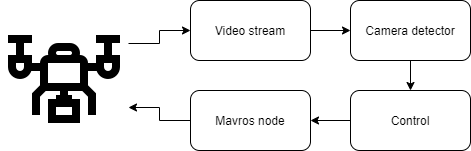
\includegraphics[width=\linewidth]{figures/local.png}
	\caption{Négy azonos konténerrel drónirányítás}
	\label{fig:azonos}
\end{figure}
A teszt architektúrája a \ref{fig:azonos}. képen látható. A teszt sikeresnek mondható, mivel a drónt sikerült irányításra bírni, illetve az optikai adatfolyamot fel tudta dolgozni az aruco kódfeldolgozó, habár aruco kódok nem voltak a szimulált világban.

\section{Két VM-en több drón szimulációja és vezérlése}
A következő teszten egy host OS-ből indított két VM-en teszteltem a több drón irányítását manuálisan. A teszthez telepítettem a VM-eken a fejezetben már felsorolt szoftvereket és környezeteket és a \ref{lst:multi}. listázásban bemutatott módon több drónt szimulációt is indítottam egy VM-en. Majd ezeket a földi irányítóállomás szimulátorával manuálisan vezéreltem. A teszt architektúrája a \ref{fig:ketvm}. ábrán látható.
\begin{figure}
	\centering
	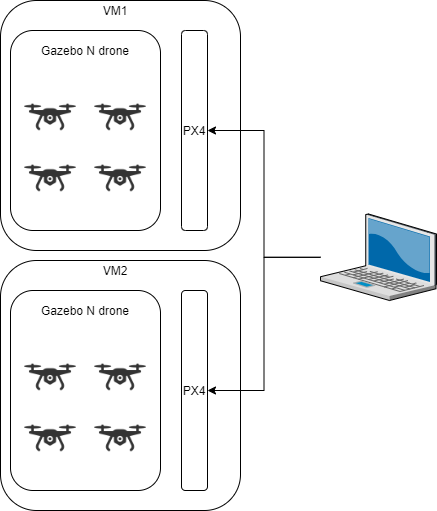
\includegraphics[height=10cm]{figures/multi-control.png}
	\caption{Két VM-en több drón irányítása}
	\label{fig:ketvm}
\end{figure}
